\documentclass{article}

% if you need to pass options to natbib, use, e.g.:
%     \PassOptionsToPackage{numbers, compress}{natbib}
% before loading neurips_2020

% ready for submission
% \usepackage{neurips_2020}

% to compile a preprint version, e.g., for submission to arXiv, add add the
% [preprint] option:
\usepackage[preprint]{neurips_2020}
\bibliographystyle{unsrtnat}

% to compile a camera-ready version, add the [final] option, e.g.:
%     \usepackage[final]{neurips_2020}

% to avoid loading the natbib package, add option nonatbib:
%     \usepackage[nonatbib]{neurips_2020}

\usepackage[utf8]{inputenc} % allow utf-8 input
\usepackage[T1]{fontenc}    % use 8-bit T1 fonts
\usepackage{graphicx}
\usepackage{hyperref}       % hyperlinks
\usepackage{url}            % simple URL typesetting
\usepackage{booktabs}       % professional-quality tables
\usepackage{amsmath}
\usepackage{amssymb}
\usepackage{amsfonts}       % blackboard math symbols
\usepackage{nicefrac}       % compact symbols for 1/2, etc.
\usepackage{microtype}      % microtypography
\usepackage{alltt}
\usepackage{listings}
\usepackage{array}
\usepackage[noline, procnumbered]{algorithm2e}
\usepackage{lmodern}
\usepackage{caption}
\usepackage{subcaption}
\usepackage{xcolor}
\newcommand\mycommfont[1]{\footnotesize\ttfamily\textcolor{gray}{#1}}
\SetCommentSty{mycommfont}


\newcommand{\secref}[1]{Section~\ref{#1}}
\newcommand{\tblref}[1]{Table~\ref{#1}}
\newcommand{\figref}[1]{Figure~\ref{#1}}
\newcommand{\thmref}[1]{Theorem~\ref{#1}}
\newcommand{\algref}[1]{Algorithm~\ref{#1}}
\newcommand{\funref}[1]{Function~\ref{#1}}
\newcommand{\listingref}[1]{Listing~\ref{#1}}

\newcommand{\eg}{{\em e.g.}}
\newcommand{\ith}{$i^{th}$}
\newcommand{\cut}[1]{}
\newcommand{\todo}[1]{{\bf\em TODO:} {{\color{red}{#1}}}}

\newcommand{\spd}{\fontfamily{cmr}\textsc{\small StratPD}}
\newcommand{\cspd}{\fontfamily{cmr}\textsc{\small CatStratPD}}
\newcommand{\xnc}{${\bf X}_{\overline{c}}$}
%\newcommand{\xnj}{${\bf X}_{\overline{j}}$}
\newcommand{\xnj}{${\bf X}_{\texttt{\char`\\}j}$}
\newcommand{\xnC}{$x_{\overline{C}}$}

%\setlist[enumerate]{itemsep=-1mm}

\title{Technical Report:\\
Partial Dependence without Model Predictions through Stratification}

\author{%
  Terence Parr \\
  University of San Francisco\\
  \texttt{parrt@cs.usfca.edu} \\
  \And
  James D. Wilson \\
  University of San Francisco\\
  \texttt{jdwilson4@usfca.edu} \\
}

\begin{document}

\maketitle

\begin{abstract}
\end{abstract}

\section{Introduction}

Partial dependence, the isolated effect of a specific variable or variables on the response variable, $y$, is important to researchers and practitioners in many disparate fields such as medicine, business, and the social sciences. For example, in medicine, researchers are interested in the relationship between an individual's demographics or clinical features and their susceptibility to illness. Business analysts at a car manufacturer might need to know how changes in their supply chain are affecting defect rates. Climate scientists are interested in how different atmospheric carbon levels affect temperature.

For an explanatory matrix, $\bf X$, with a single variable, $x_1$, a plot of the $y$ against $x_1$ visualizes the marginal effect of feature $x_1$ on $y$ exactly. Given two or more features, one can similarly plot the marginal effects of each feature separately, however, the analysis is complicated by the interactions of the variables.   Variable interactions, codependencies between features, result in marginal plots that do not isolate the specific contribution of a feature of interest to the target. For example, a marginal plot of sex (male/female) against body weight would likely show that, on average, men are heavier than women. While true, men are also taller than women on average, which likely accounts for most of the difference in average weight. It is unlikely that two ``identical'' people, differing only in sex, would be appreciably different in weight.  

Rather than looking directly at the data, there are several partial dependence techniques that interrogate fitted models provided by the user: Friedman's original partial dependence (which we will denote FPD) \citet{PDP}, Individual Conditional Expectations (ICE) \citet{ICE}, Accumulated Local Effects (ALE) \citet{ALE}, and most recently SHAP \citet{shap}.  Model-based techniques dominate the partial dependence research literature because interpreting the output of a fitted model  has several advantages. Models have a tendency to smooth over noise. Models act like analysis preprocessing steps, potentially reducing the computational burden on model-based partial dependence techniques; e.g., ALE is $O(n)$ for the $n$ records of $\bf X$. Model-based techniques are typically model-agnostic, though for efficiency, some provide model-specific optimizations, as SHAP does. Partial dependence techniques that interrogate models also provide insight into the models themselves; i.e., how variables affect model behavior.  It is also true that, in some cases, a predictive model is the primary goal so creating a suitable model is not an extra burden.

Model-based techniques do have some significant disadvantages, however.   As we demonstrate in \secref{sec:experiments} using synthetic and real data sets, model-based techniques vary in their ability to tease apart the effect of codependent features on the response.  Also, recall that there are vast armies of business analysts and scientists at work that need to analyze data, in a manner akin to exploratory data analysis (EDA), that have no intention of creating a predictive model.  Either they have no need, perhaps needing only partial dependence plots, or they do not have the expertise to choose, tune, and assess models (or write software at all). 

\begin{figure}
\begin{center}
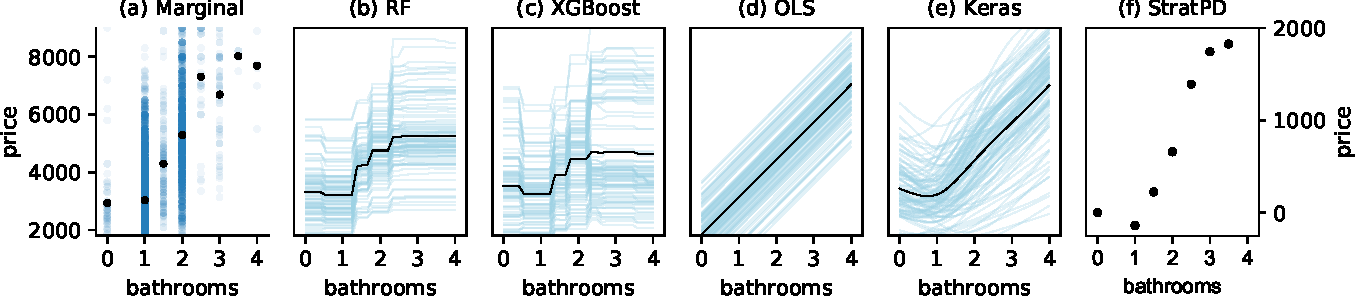
\includegraphics[scale=0.61]{images/bathrooms_vs_price.pdf}
\caption{\small Plots of bathrooms versus rent price using New York City apartment rent data. (a) marginal plot, (b) PD/ICE plot derived from random forest, (c) PD/ICE plot derived from gradient boosted machine, and (d) PD/ICE plot derived from ordinary least squares regression; sample size is 10,000 observations of \textasciitilde50k. The PD/ICE plots are  different for the same data set, depending on the chosen user model. X['bathrooms'].unique() shows (array([0. , 1. , 1.5, 2. , 2.5, 3. , 3.5, 4. ]),
 array([  54, 8151,  140, 1539,   39,   67,    3,    7])). \spd{} has missing last value, not enough data. what are $R^2$ values. how tuned \vspace{-7mm}}
\label{fig:baths_price}
\end{center}
\end{figure}

Even in the case where a machine learning practitioner is available to create a fitted model for the analyst, hazards exist. First, if a fitted model is unable to accurately capture the relationship between features and $y$ accurately, for whatever reason, then partial dependence does not provide any useful information to the user.  To make interpretation more challenging, there is no definition of ``accurate enough.'' Second, given an accurate fitted model, business analysts and scientists are still peering at the data through the lens of the model, which can distort partial dependence curves. Separating visual artifacts of the model from real effects present in the data requires expertise in model behavior (and optimally in the implementation of model fitting algorithms). 

Consider the combined FPD/ICE plots shown in \figref{fig:baths_price} derived from several models (random forest, gradient boosting, linear regression, deep learning) fitted to the same New York City rent data set \citet{rent}.  The subplots in \figref{fig:baths_price}(b)-(e)  present starkly different partial dependence relationships and it is unclear which, if any, is correct.  The marginal plot, (a), drawn directly from the data shows a roughly linear growth in price for a rise in the number of bathrooms, but this relationship is biased because of the dependence of bathrooms on other variables, such as the number of bedrooms. (e.g., five bathroom, one bedroom apartments are unlikely.)  For real data sets with codependent features, the true relationship is unknown so it is hard to evaluate the correctness of the plots. (Humans are unreliable estimators, which is why we need data analysis algorithms in the first place.) Nonetheless, having the same algorithm, operating on the same data, give meaningfully different partial dependences is undesirable and makes one question their validity.

Experts are often able to quickly recognize model artifacts, such as the stairstep phenomenon inherent to the decision tree-based methods in \figref{fig:baths_price}(b) and (c).  In this case, though, the stairstep is more accurate than the linear relationship in (d) and (e) because the number of bathrooms is discrete (except for ``half baths'').  The point is that interpreting model-based partial dependence plots can be misleading, even for experts. 

An accurate mechanism to compute partial dependences that did not peer through fitted models would be most welcome.  Such partial dependence curves would be accessible to users, like business analysts, who lack the expertise to create suitable models and would also reduce the chance of plot misinterpretation due to model artifacts. The curves could also help machine learning practitioners to choose appropriate models based upon relationships exposed in the data.

In this paper, we propose a strategy, called {\textsc{strat}ified \textsc{p}artial \textsc{d}ependence} (\spd{}), that ({\it i}) computes partial dependences directly from training data $({\bf X}, {\bf y})$, rather than through the predictions of a fitted model, and ({\it ii}) does not presume mutually-independent features.  As an example, \figref{fig:baths_price}(f) shows the partial dependence plot computed by \spd. The technique depends on the notion of an idealized partial dependence:  integration over the partial derivative of $y$ with respect to the variable of interest for the smooth function that generated $({\bf X}, {\bf y})$. As that function is unknown, we estimate the partial derivatives from the data non-parametrically.  Colloquially, the approach examines changes in $y$ across $x_j$ while holding \xnj{} constant or very similar (\xnj{} denotes all variables except $x_j$). A similar stratification approach works for categorical variables (\cspd). Both \spd{} and \cspd{} have $O(n^2)$ worst-case time complexity (like FPD), but \spd{} behaves linearly on real data sets.  Our prototype is currently limited to regression, isolates only single-variable partial dependence, and cannot identify interaction effects (as ICE can).  The software is available via Python package {\tt stratx} with source code at {\tt github}, including the code to regenerate images in this paper.

We begin by describing and providing algorithms for the proposed stratification approach in \secref{sec:stratpd} then compare \spd{} to related (model-based) work in \secref{sec:related}. In \secref{sec:experiments}, we present partial dependence curves generated by \spd{} and \cspd{} on real data sets, contrast the plots with those of existing methods, and use synthetic data to highlight biases in some model-based methods.

\section{Partial dependence without model predictions}\label{sec:stratpd}


To estimate partial derivatives, \spd{} stratifies \xnj{} feature space  into disjoint regions of observations where all \xnj{} variables are approximately matched across the observations in that region. Within each \xnj{} region, any fluctuations in the response variable are likely due to the variable of interest, $x_j$.  Estimates of the partial derivative within a region are computed discretely via the changes in $y$ values between unique $x_j$ positions. The overall partial derivative at $x_j=z$ is the average of all slopes, found in any region, whose $x_j$ range spans $z$.  Stratification occurs through the use of a decision tree but only for the purpose of partitioning feature space; \spd{} never uses predictions from any model.



\noindent {\bf Definition 1} The {\em idealized partial dependence} of $y$ on feature $x_j$ for smooth generator function $f:\mathbb{R}^{p} \rightarrow \mathbb{R}$ evaluated at $x_j = z$ is the cumulative sum up to $z$:

\begin{equation}\label{eq:pd}
\text{\it PD}_j(z) = \int_{min(x_j)}^z \frac{\partial y}{\partial x_j} dx_j
\end{equation}

$\text{\it PD}_j(z)$ is the value contributed to $y$ by $x_j$ at $x_j = z$ and $\text{\it PD}_j(min(x_j))=0$. The advantages of this partial dependence definition are that it does not depend on predictions from a fitted model and is insensitive to collinear or otherwise codependent features, unlike the Friedman's original definition that he points out is less accurate for codependent data sets. We will denote Friedman's as $\text{\it FPD}_j$ to distinguish it from this ideal, $\text{\it PD}_j$.

For example, consider quadratic equation $y = x_1^2 + x_2 + 100$ as a generator of data in $[0,3]$. The partial derivatives are $\frac{\partial y}{\partial x_1} = 2 x_1$ and $\frac{\partial y}{\partial x_2} = 1$, giving $\text{\it PD}_1 = x_1^2$ and $\text{\it PD}_2 = x_2$. 

The obvious disadvantage of this feature impact definition is that function $f$, from which $\text{\it PD}_j$ is derived, is unknown in practice, so symbolically computing the partial derivatives is not possible. But, if we could compute accurate partial dependence curves by some other method, then this definition would still represent a viable means to obtain feature impacts. 

\spd{} stratifies a data set into groups of observations that are similar, except in the variable of interest, $x_j$, through the use of a single decision tree. Any fluctuation of the response variable within a group (decision tree leaf) is likely due to $x_j$.  The $\beta_1$ coefficient of a simple local linear regression fit to the $(x_j, y)$ values within a group provides an estimate of $\frac{\partial y}{\partial x_j}$ in that group's $x_j$ range. Averaging the partial derivative estimates across all such groups yields the overall $\frac{\partial y}{\partial x_j}$ partial derivative approximation. The cumulative sum of the estimated partial derivative yields the partial dependence curve. 

{\bf StratPD}\begin{alltt}\small
Fit tree regressor to all but x_c with hyper parameter min_slopes_per_x
For each leaf:
    y bar = Group leaf samples by x_c, computing average y per unique x_c
    dx = discrete difference between adjacent unique x_c
    dy = discrete difference between adjacent average y bar
    add (x[i], x[i+1], dy[i]/dx[i]) for each unique x_c to list D

for each x in unique x_c from X:
    slopes = [slope for (a, b, slope) in D if x >= a and x < b]
    count[x] = |slopes|
    dydx[x] = mean(slopes)

Drop slope estimates computed using fewer than min_slopes_per_x values
pdx = discrete difference between adjacent unique x_c
pdy = cumulative sum of dydx * pdx
return pdx, [0]+pdy  // insert 0 for pdx[0] since sum contributed from beyond left is 0
\end{alltt}

{\bf CatStratPD}\begin{alltt}\small
Fit tree regressor to all but x_c with hyper parameter min_slopes_per_x
For each leaf:
    y bar = Group leaf samples by categories of x_c, computing average y per unique category x_c
    Compute unique categories and counts per category
    refcat is randomly chosen category from x_c
    For each unique category x in leaf:
        delta[cat,leaf] = Subtract y for refcat from all y bar (refcat delta will be 0)
end
Let Avg[cat] be vector with running sum mapping category to count
work = set of leaf indexes
while more work and something changed and less than max iterations:
    for each leaf in leaves:
        if cat in delta[:,leaf] intersects with Avg:
            j = random category in intersection
            adjust delta[:,leaf] to be relative to j so delta[j,leaf]==0 then add Avg[j] so comparable
            merge into Avg
    work -= all j merged this iteration
\end{alltt}

\section{Related work}\label{sec:related}

FPD

ICE

ALE

SHAP

cold start, counting execution time and number of hyper parameters. particularly deep learning

The techniques differ in algorithm simplicity, performance, and ability to isolate codependent variables. a nonparametric technique could also inform which machine learning model to use if a model is desired.

SHAP is mean centered FPD for independent variables, proof in supplemental material.

\section{Experimental results}\label{sec:experiments}

what if X,y relationship is very weak? models would get low accuracy. what happens to us?  I think we would simply show low partial dependence curves.

\begin{figure}[htbp]
\begin{center}
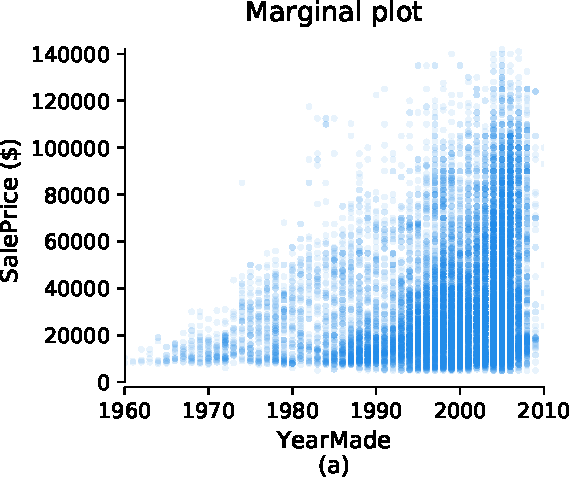
\includegraphics[scale=0.35]{images/bulldozer_YearMade_marginal.pdf}~~
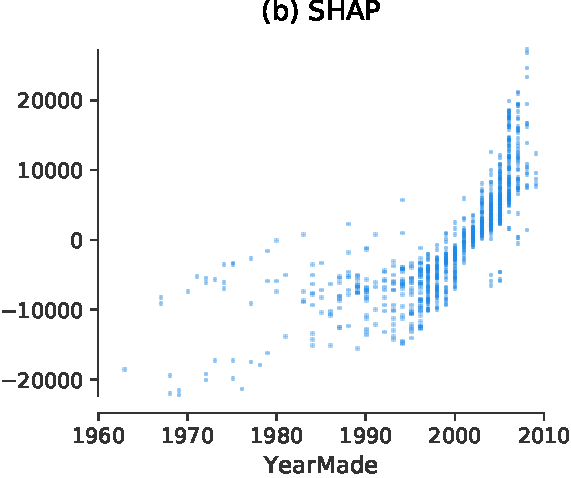
\includegraphics[scale=0.35]{images/bulldozer_YearMade_shap.pdf}~~
\includegraphics[scale=0.35]{images/YearMade_400_ale.pdf}~~
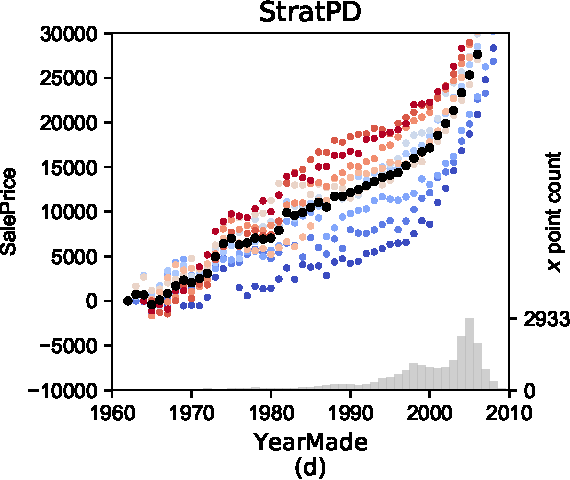
\includegraphics[scale=0.35]{images/bulldozer_YearMade_stratpd.pdf}
\caption{\small (a) Marginal plot of bulldozer {\tt YearMade} versus {\tt SalePrice} using subsample of 20k observations, (b) partial dependence drawn by SHAP interrogating an RF with 40 trees and explaining 1000 values with 100 observations as background data, (c) \spd{} partial dependence.}
\label{fig:shap-stratpd-YearMade}
\end{center}
\end{figure}

\begin{figure}[htbp]
\begin{center}
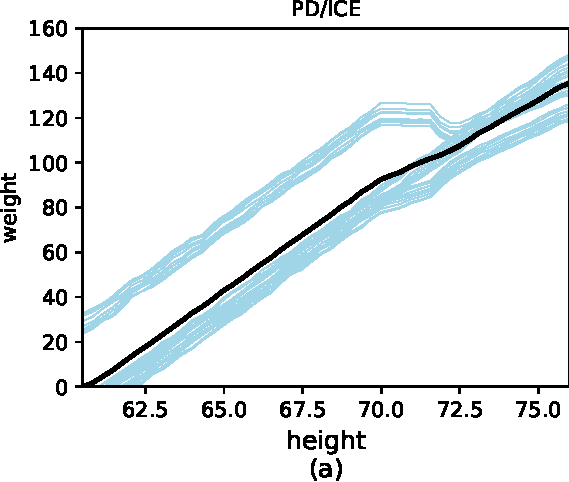
\includegraphics[scale=0.35]{images/height_vs_weight_pdp.pdf}~~
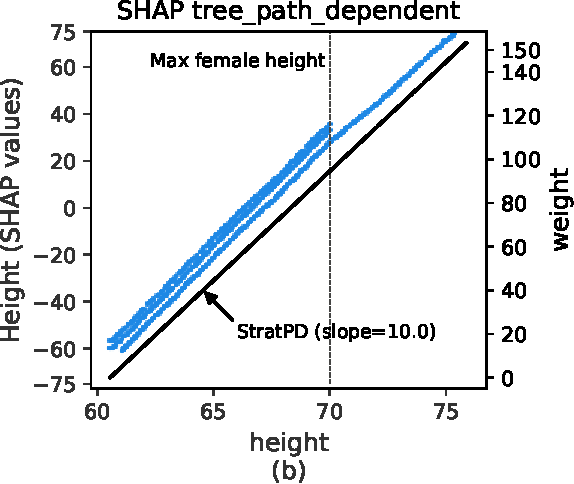
\includegraphics[scale=0.35]{images/weight_tree_path_dependent_shap.pdf}~~
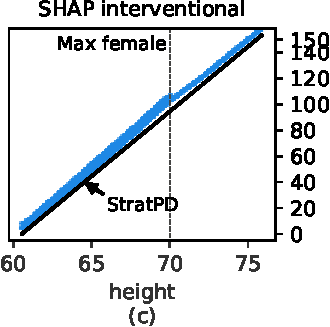
\includegraphics[scale=0.35]{images/weight_interventional_shap.pdf}~~
\includegraphics[scale=0.34]{images/height_300_ale.pdf}~~
\caption{\small SHAP partial dependence plots of response body weight on feature {\tt height} using 2000 synthetic observations from Equation \eqref{eq:weight}. SHAP interrogated an RF with 40 trees and explained all 2000 samples; the interventional case used 100 observations as background data.}
\label{fig:heightweight}
\end{center}
\end{figure}

\begin{figure}[htbp]
\begin{center}
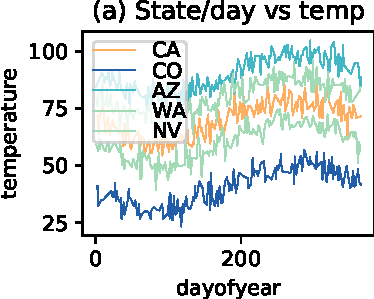
\includegraphics[scale=0.45]{images/dayofyear_vs_temp.pdf}~~
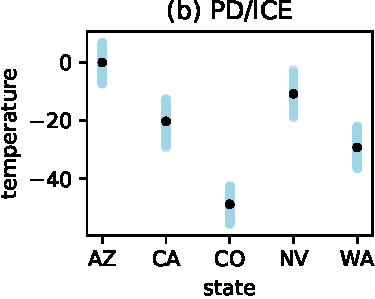
\includegraphics[scale=0.45]{images/state_vs_temp_pdp.pdf}~~
\includegraphics[scale=0.45]{images/state_5_ale.pdf}~~
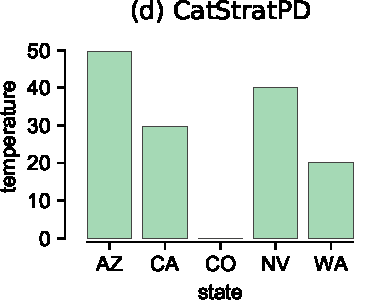
\includegraphics[scale=0.45]{images/state_vs_temp_stratpd.pdf}~~
\caption{\small foo.}
\label{fig:statetemp}
\end{center}
\end{figure}

\begin{figure}[htbp]
\begin{center}
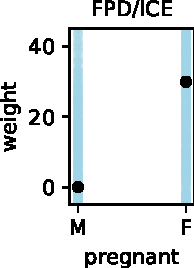
\includegraphics[scale=0.45]{images/pregnant_vs_weight_pdp.pdf}~~
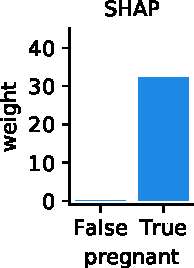
\includegraphics[scale=0.45]{images/pregnant_vs_weight_shap.pdf}~~
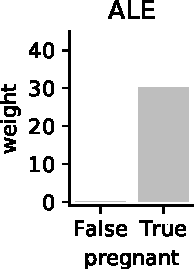
\includegraphics[scale=0.45]{images/pregnant_2_ale.pdf}~~
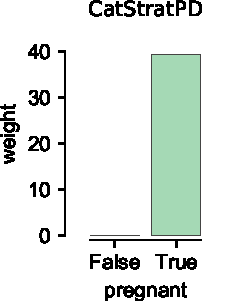
\includegraphics[scale=0.45]{images/pregnant_vs_weight_stratpd.pdf}~~
\caption{\small foo.}
\label{fig:pregnant}
\end{center}
\end{figure}

\begin{figure}[htbp]
\begin{center}
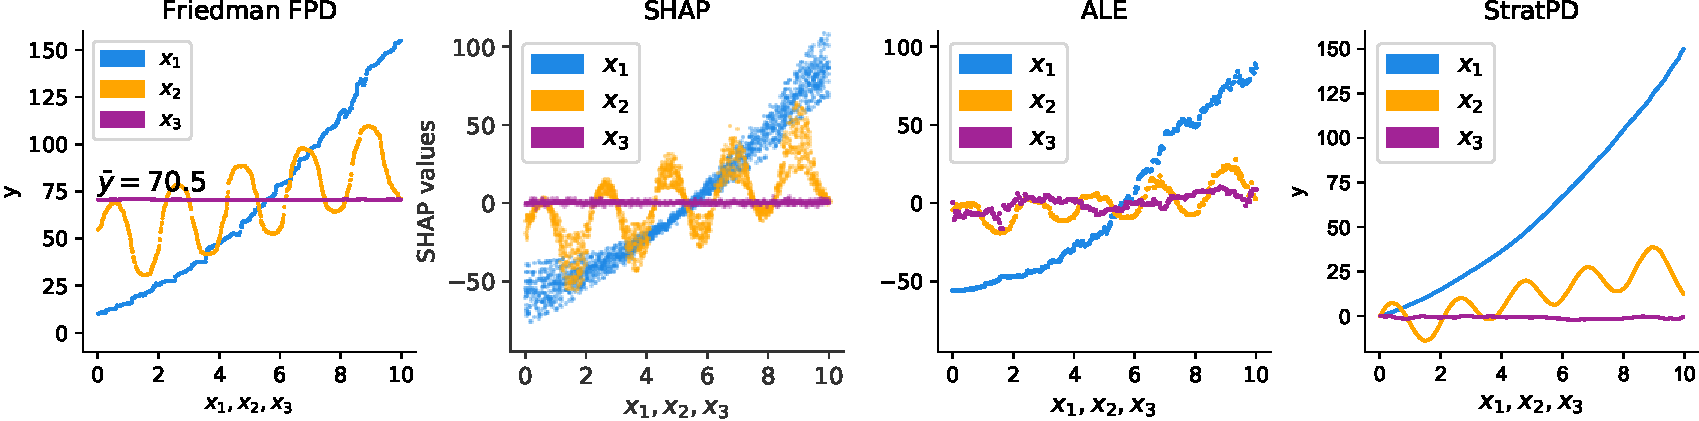
\includegraphics[scale=0.4]{images/interactions.pdf}
\caption{\small $y = x_1^2 + x_1 x_2 + 5 x_1 sin(3 x_2) + 10$ where $x_1,x_2,x_3 \sim U(0,10)$ and $x_3$ does not affect $y$. No noise added.}
\label{fig:interactions}
\end{center}
\end{figure}

\begin{figure}[htbp]
\begin{center}
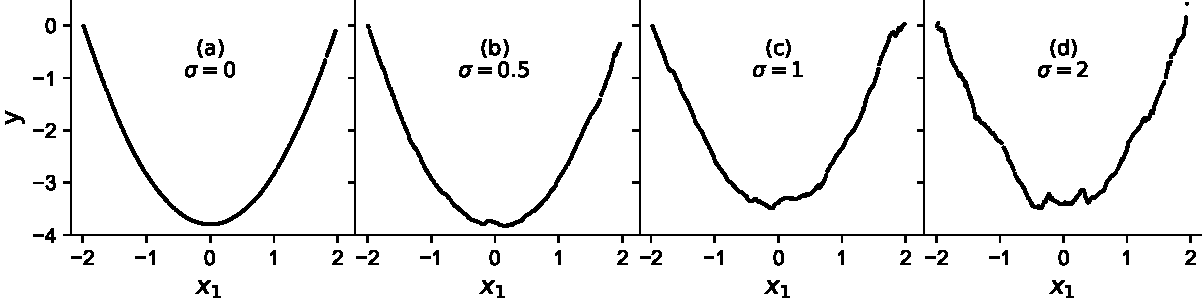
\includegraphics[scale=0.4]{images/noise.pdf}
\caption{\small $y = x_1^2 + x_1 + 10 + N(0,\sigma)$ where $x_1,x_2 \sim U(-2,2)$ and $\sigma \in [0,0.5,1,2]$.}
\label{fig:noise}
\end{center}
\end{figure}

\section{Discussion and future work}

\pagebreak
\section{Appendix}

\setlength{\algomargin}{5pt}
\begin{algorithm}[]
\DontPrintSemicolon
\SetAlgorithmName{Algorithm}{List of Algorithms}
\SetAlgoSkip{}
\TitleOfAlgo{{\em StratPD}}
\KwIn{{\bf X}, {\bf y}, c, {\it min\_samples\_leaf}, {\it min\_slopes\_per\_x}}
\KwOut{$\bf pdx, pdy$: Unique $x_c$, partial dependence values across $x_c$}
$T$ := Decision tree regressor fit to (\xnc{}, $\bf y$) with hyper-parameter: ${\it min\_samples\_leaf}$\;
\For{each leaf $l \in T$}{
        $({\bf x}_l, {\bf y}_l)$ = $\{(x_c^{(i)},  y^{(i)})\}_{i \in l}$\tcp*{\it Get leaf samples}
        {\bf ux} := $unique({\bf x}_l)$\\
	$\bar{\bf y}$ := Group leaf records $({\bf x}_l, {\bf y}_l)$ by value of ${\bf x}_l$, computing $\bar{y}$ per unique value\\
	${\bf dx}$ := ${\bf ux}^{(i+1)} - {\bf ux}^{(i)}_{i=1..|{\bf ux}|-1}$\tcp*{\it Discrete difference}
	${\bf dy}$ := $\bar{\bf y}^{(i+1)} - \bar{\bf y}^{(i)}_{i=1..|{\bf ux}|-1}$\\
	Add tuples ${({\bf ux}^{(i)}, {\bf ux}^{(i+1)},~ {\bf dy}^{(i)}/{\bf dx}^{(i)})}_{i=1..|{\bf ux}|-1}$ to list ${\bf d}$\\
}
$\bf ux$ := $unique(\{x_c^{(i)}\}_{i=1..n})$\\
\For{each $x \in {\bf ux}$\tcp*{\it Counts slopes, compute average slope per unique $x_c$ value}}{
	$slopes$ := [$slope$ for $(a,b,slope) \in \bf d$ if $x \ge a$ and $x <b$]\\
	${\bf c}_x$ := $|slopes|$\\
	${\bf dydx}_x$ := $\overline{slopes}$\\
}
${\bf dydx}$ := ${\bf dydx}[{\bf c} \ge min\_slopes\_per\_x]$\tcp*{\it Drop slope estimates computed from too few}
${\bf ux}$ := ${\bf ux}[{\bf c} \ge min\_slopes\_per\_x]$\\
$\bf pdx$ := ${\bf ux}^{(i+1)} - {\bf ux}^{(i)}_{i=1..|{\bf ux}|-1}$\\
$\bf pdy$ := [0] + cumulative\_sum(${\bf dydx} * \bf pdx$)~~~\tcp*{\it integrate, inserting 0 for leftmost $x_c$}
\Return{$\bf pdx, pdy$}
\label{alg:CatStratPD}
\end{algorithm}

\setlength{\algomargin}{5pt}
\begin{algorithm}[]
\DontPrintSemicolon
\SetAlgorithmName{Algorithm}{List of Algorithms}
\SetAlgoSkip{}
\TitleOfAlgo{{\em CatStratPD}}
\KwIn{${\bf X}, {\bf y}, c, {\it min\_samples\_leaf}$}
\KwOut{$\begin{array}[t]{l}
\Delta^{(k)} = \text{category } k \text{'s effect on } y \text{ where } mean(\Delta^{(k)})=0\\
n^{(k)} = \text{number of supported observations per category $k$}\\
\end{array}$
}
$T$ := Decision tree regressor fit to (\xnc{}, $\bf y$) with hyper-parameter: ${\it min\_samples\_leaf}$\;
\tcp{\it Get average $y$ delta relative to random ref category for each sample in each leaf}
Let $\Delta_{x,l}$ be dictionary mapping (category, leaf) to delta from ref category\\
Let ${\it Count}_{x,l}$ be dictionary mapping (category, leaf) to count\\
\For{each leaf $l \in T$}{
        $({\bf x}_l, {\bf y}_l)$ = $\{(x_c^{(i)},  y^{(i)})\}_{i \in l}$\tcp*{\it Get leaf samples}
        ${\bf ux}$, ${\bf cx}$ := $unique({\bf x}_l)$\tcp*{\it Get unique categories, counts from leaf samples}
	$\bar{\bf y}$ := Group leaf records $({\bf x}_l, {\bf y}_l)$ by categories of ${\bf x}_l$, computing $\bar{y}$ per unique category\\
	${\it refcat}_l$ := random category from ${\bf y}$\\
%	$y_{\it ref}$ := random choice from $\bar{\bf y}$\\
	\For{each $x \in {\bf ux}$}{
		${\it Count}_{x,l}$ := ${\bf cx}_x$\\
        		$\Delta_{x,l}$ := $\bar{\bf y} - y[{\it refcat}_l]$\\
	}
}
work := 1 .. $|uniq\_refcats|$\\
Let $Avg_x$ be vector with running sum mapping category to count\\
\While{len(work) > 0 and len(completed)>0 and iteration<=max\_iter}{
}
\label{alg:CatStratPD}
\end{algorithm}


{\small
\bibliography{stratpd}
}
\end{document}